% ============================================================
% Bao cao BTL CO4031 - Phan cua Nguoi A (Data & DW)
% Bien dich:  xelatex part_A_dw.tex   (chay 2 lan de co muc luc)
% ============================================================
\documentclass[12pt,a4paper]{article}

\usepackage{fontspec}
\setmainfont{Latin Modern Roman}
\setmonofont{DejaVu Sans Mono}[Scale=0.82]
\usepackage[a4paper,margin=2.5cm]{geometry}
\usepackage{setspace}
\onehalfspacing
\usepackage{booktabs,longtable,tabularx,array}
\usepackage{graphicx}
\usepackage{xcolor}
\usepackage{listings}
\usepackage{enumitem}
\usepackage{caption}
\usepackage{tikz}
\usetikzlibrary{arrows.meta,positioning,shapes.geometric}
\usepackage[colorlinks=true,linkcolor=blue!50!black,urlcolor=blue!50!black]{hyperref}

% --- Tieu de tieng Viet ---
\renewcommand{\contentsname}{Mục lục}
\renewcommand{\figurename}{Hình}
\renewcommand{\tablename}{Bảng}
\renewcommand{\listfigurename}{Danh mục hình}
\renewcommand{\listtablename}{Danh mục bảng}
\renewcommand{\refname}{Tài liệu tham khảo}

% --- Code listing ---
\definecolor{codebg}{RGB}{245,245,245}
\lstdefinestyle{sql}{
  language=SQL, basicstyle=\ttfamily\footnotesize, backgroundcolor=\color{codebg},
  keywordstyle=\color{blue!60!black}\bfseries, commentstyle=\color{green!40!black},
  breaklines=true, frame=single, rulecolor=\color{black!20}, showstringspaces=false,
  morekeywords={CASE,WHEN,THEN,ELSE,END,LIMIT,PRAGMA,AUTOINCREMENT,REFERENCES,IF,EXISTS}
}
\lstdefinestyle{py}{
  language=Python, basicstyle=\ttfamily\footnotesize, backgroundcolor=\color{codebg},
  keywordstyle=\color{blue!60!black}\bfseries, commentstyle=\color{green!40!black},
  breaklines=true, frame=single, rulecolor=\color{black!20}, showstringspaces=false
}
\newcommand{\code}[1]{\texttt{\small #1}}
\captionsetup{font=small,labelfont=bf}

\title{\textbf{BÁO CÁO BÀI TẬP LỚN CO4031}\\[4pt]
\Large Kho dữ liệu thương mại điện tử Olist và hệ hỗ trợ ra quyết định\\[4pt]
\large Phần A: Phân tích yêu cầu, thiết kế kho dữ liệu, ETL và OLAP}
\author{Người phụ trách: tamnguyen635 (Người A -- Data \& DW)}
\date{Học kỳ 261 -- Năm học 2026--2027}

\begin{document}
\maketitle
\tableofcontents
\clearpage

% ============================================================
\section{Giới thiệu và phân tích yêu cầu nghiệp vụ}
% ============================================================

\subsection{Bối cảnh bài toán}
Thương mại điện tử sinh ra lượng dữ liệu giao dịch rất lớn: mỗi đơn hàng gắn với khách hàng, người bán,
sản phẩm, hình thức thanh toán, thời gian giao hàng và đánh giá sau mua. Các hệ thống tác nghiệp (OLTP)
lưu những dữ liệu này theo dạng chuẩn hóa để xử lý giao dịch nhanh, nhưng \emph{không} thuận tiện cho việc
phân tích tổng hợp theo nhiều chiều (thời gian, vùng, danh mục\ldots). Vì vậy cần một kho dữ liệu
(Data Warehouse -- DW) tích hợp dữ liệu lịch sử và một hệ hỗ trợ quyết định (DSS) khai thác kho đó.

Nhóm chọn lĩnh vực \textbf{bán lẻ / thương mại điện tử}, dùng bộ dữ liệu công khai
\emph{Brazilian E-Commerce Public Dataset by Olist} (Kaggle) \cite{olist}. Bộ dữ liệu gồm khoảng 100 nghìn đơn hàng thật
đã được ẩn danh, từ 04/09/2016 đến 17/10/2018, đáp ứng yêu cầu về quy mô và ý nghĩa thực tế của đề bài.

\subsection{Đối tượng sử dụng và câu hỏi nghiệp vụ}
Kho dữ liệu phục vụ ban quản lý của một sàn thương mại điện tử (quản lý kinh doanh, vận hành, chăm sóc
khách hàng). Các câu hỏi nghiệp vụ chính mà phần DW phải trả lời được:

\begin{enumerate}[nosep]
  \item Doanh thu thay đổi thế nào theo năm, quý, tháng? Thời điểm nào là cao điểm?
  \item Danh mục sản phẩm nào đóng góp nhiều doanh thu nhất, và xu hướng của chúng qua các năm ra sao?
  \item Doanh thu và mức độ hài lòng của khách phân bố theo bang/vùng như thế nào?
  \item Khách hàng thanh toán bằng hình thức nào, có trả góp hay không?
  \item Giao hàng trễ ảnh hưởng thế nào đến điểm đánh giá của khách?
\end{enumerate}

Các câu hỏi này là đầu vào cho thành phần DSS (phần B): dự báo doanh thu, phân khúc khách hàng và mô hình
what-if cho vận hành.

\subsection{Nguồn dữ liệu}
Dữ liệu nguồn gồm 8 tệp CSV có quan hệ với nhau, mô phỏng một cơ sở dữ liệu tác nghiệp (Bảng~\ref{tab:sources}).
Tệp \code{olist\_geolocation\_dataset} (khoảng 1 triệu dòng tọa độ theo mã bưu chính) không được dùng vì
thành phố, bang và mã bưu chính đã có sẵn trong tệp khách hàng và người bán, đủ cho các phân tích theo địa lý.

\begin{table}[h]
\centering
\caption{Các tệp dữ liệu nguồn}\label{tab:sources}
\small
\begin{tabularx}{\textwidth}{@{}l r X@{}}
\toprule
\textbf{Tệp} & \textbf{Số dòng} & \textbf{Nội dung chính}\\
\midrule
\code{olist\_orders} & 99.441 & Đơn hàng: trạng thái, ngày mua, ngày giao thực tế, ngày giao dự kiến\\
\code{olist\_order\_items} & 112.650 & Từng sản phẩm trong đơn: sản phẩm, người bán, giá, phí vận chuyển\\
\code{olist\_customers} & 99.441 & Khách hàng: mã khách, thành phố, bang, mã bưu chính\\
\code{olist\_products} & 32.951 & Sản phẩm: danh mục, kích thước, cân nặng, số ảnh\\
\code{olist\_sellers} & 3.095 & Người bán: thành phố, bang\\
\code{olist\_order\_payments} & 103.886 & Thanh toán: hình thức, số kỳ trả góp, số tiền\\
\code{olist\_order\_reviews} & 99.224 & Đánh giá: điểm 1--5, bình luận\\
\code{product\_category\_name\_translation} & 71 & Dịch tên danh mục từ tiếng Bồ Đào Nha sang tiếng Anh\\
\bottomrule
\end{tabularx}
\end{table}

\subsection{Kết quả khảo sát chất lượng dữ liệu}
Trước khi thiết kế, nhóm khảo sát toàn bộ 8 tệp. Những phát hiện ảnh hưởng trực tiếp đến thiết kế và ETL:

\begin{itemize}[nosep]
  \item Khóa tham chiếu \emph{toàn vẹn}: mọi \code{order\_id}, \code{product\_id}, \code{seller\_id},
        \code{customer\_id} trong bảng chi tiết đơn đều tồn tại ở bảng gốc.
  \item \code{customer\_id} \emph{thay đổi theo từng đơn hàng}; người mua thật được xác định bằng
        \code{customer\_unique\_id} (96.096 người trên 99.441 mã).
  \item 775 đơn hàng không có sản phẩm nào (chủ yếu đơn đã hủy hoặc chưa hoàn tất).
  \item 2.246 đơn thanh toán bằng nhiều hình thức; 547 đơn có nhiều hơn một đánh giá; 1 đơn không có thanh toán.
  \item 610 sản phẩm không có danh mục; 2 danh mục (\code{pc\_gamer}, bếp di động) thiếu bản dịch.
  \item Giá trị thiếu hợp lý về nghiệp vụ: đơn chưa giao thì chưa có ngày giao; nhiều đơn không có bình luận.
  \item 8 đơn ở trạng thái \emph{delivered} nhưng thiếu ngày giao; 6 đơn chưa ở trạng thái \emph{delivered} nhưng đã có ngày giao.
\end{itemize}

% ============================================================
\section{Thiết kế kho dữ liệu}
% ============================================================

\subsection{Kiến trúc tổng thể}
Hệ thống theo kiến trúc ba tầng của kho dữ liệu: tầng nguồn (CSV), tầng tích hợp/ETL và tầng kho dữ liệu đa chiều,
trên đó là tầng trình bày (OLAP, dashboard, DSS). Hình~\ref{fig:arch} minh họa luồng dữ liệu.

\begin{figure}[h]
\centering
\begin{tikzpicture}[
  node distance=9mm,
  box/.style={draw, rounded corners, minimum height=1.1cm, minimum width=2.6cm, align=center, fill=blue!6},
  arr/.style={-{Latex[length=2.5mm]}, thick}]
  \node[box] (src) {Nguồn\\8 tệp CSV Olist};
  \node[box, right=of src] (etl) {ETL\\Python / pandas};
  \node[box, right=of etl, fill=orange!15] (dw) {Kho dữ liệu\\SQLite (star schema)};
  \node[box, right=of dw, fill=green!10] (use) {OLAP, Dashboard,\\DSS};
  \draw[arr] (src) -- (etl);
  \draw[arr] (etl) -- (dw);
  \draw[arr] (dw) -- (use);
\end{tikzpicture}
\caption{Luồng dữ liệu của hệ thống}\label{fig:arch}
\end{figure}

\subsection{Lựa chọn phương pháp và công nghệ}
Theo hai trường phái kinh điển, Inmon xây kho dữ liệu doanh nghiệp (EDW) chuẩn hóa trước rồi tách ra các
data mart (top-down), còn Kimball xây từng data mart theo mô hình chiều rồi hợp nhất dần (bottom-up)
\cite{kimball2013,inmon2005}. Nhóm chọn \textbf{hướng Kimball với một data mart cho chủ đề bán hàng}, vì:
(i) bài toán có phạm vi một quy trình nghiệp vụ rõ ràng (bán hàng); (ii) thời gian thực hiện ngắn, cần giá trị
sử dụng sớm; (iii) mô hình chiều dạng sao tối ưu cho truy vấn tổng hợp và dễ hiểu với người dùng nghiệp vụ.

Về công nghệ, nhóm dùng \textbf{SQLite} làm hệ quản trị lưu kho, theo kiểu \textbf{ROLAP}: các phép OLAP
được thực hiện bằng truy vấn SQL trên lược đồ quan hệ, không dựng khối dữ liệu (cube) được tính trước như
MOLAP. SQLite gọn, chạy cục bộ và đủ nhanh cho khoảng 112 nghìn dòng fact.

\subsection{Mức hạt (granularity)}
Mức hạt của bảng fact là \textbf{một dòng cho mỗi sản phẩm trong một đơn hàng}
(\code{order\_id} + \code{order\_item\_id}). Đây là mức chi tiết nhất có sẵn trong nguồn: từ đó có thể
cộng dồn lên theo đơn, theo ngày, theo danh mục, theo bang\ldots mà không mất thông tin. Chọn mức hạt thấp hơn
(ví dụ gộp theo đơn) sẽ làm mất khả năng phân tích theo sản phẩm và người bán, vì một đơn có thể chứa nhiều sản phẩm
từ nhiều người bán khác nhau. Chi phí là số dòng fact lớn hơn, nhưng với quy mô này là hoàn toàn chấp nhận được.

\subsection{Mô hình dữ liệu đa chiều}
Lược đồ là \textbf{star schema} gồm một bảng fact \code{fact\_sales} và sáu bảng chiều (Hình~\ref{fig:star}).

\begin{figure}[h]
\centering
\IfFileExists{figures/star_schema.pdf}{%
  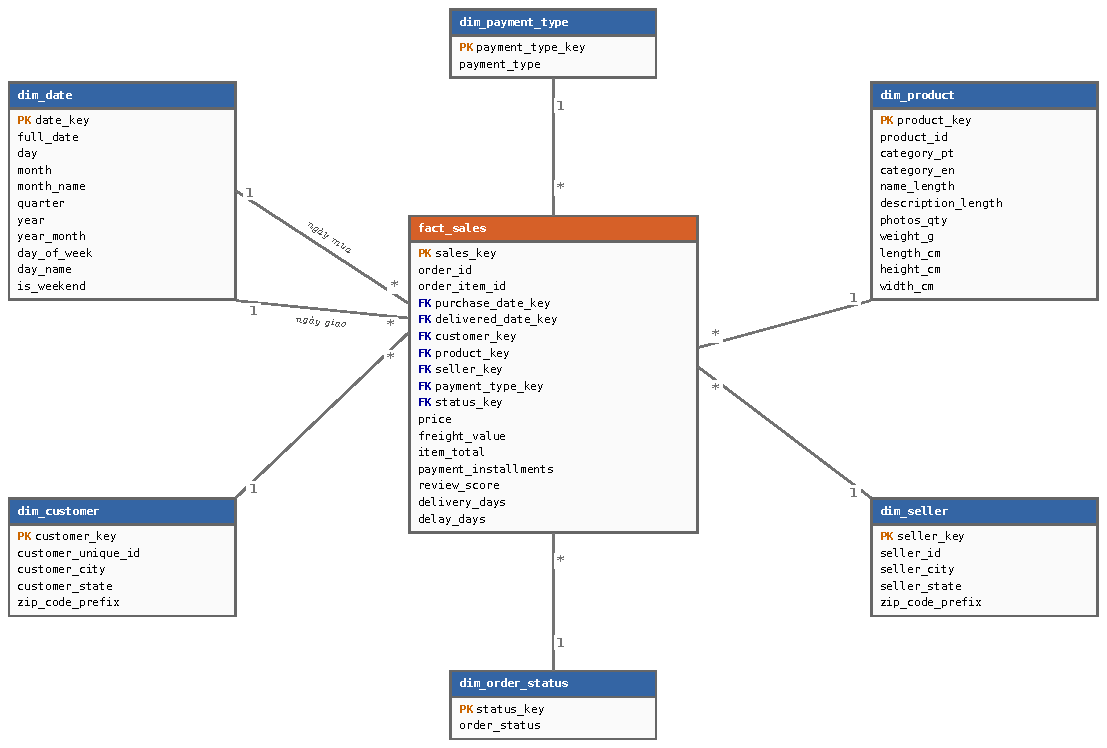
\includegraphics[width=\textwidth]{figures/star_schema.pdf}}{%
  \fbox{\parbox{0.9\textwidth}{\centering\vspace{2cm}\textit{Sơ đồ star schema sẽ được bổ sung}\vspace{2cm}}}}
\caption{Star schema của kho dữ liệu bán hàng Olist}\label{fig:star}
\end{figure}

\paragraph{Bảng fact \code{fact\_sales}.}
Chứa khóa ngoại tới các chiều, một chiều suy biến (\code{order\_id}) và các độ đo (Bảng~\ref{tab:fact}).

\begin{table}[h]
\centering
\caption{Các cột của bảng fact}\label{tab:fact}
\small
\begin{tabularx}{\textwidth}{@{}l l X@{}}
\toprule
\textbf{Cột} & \textbf{Loại} & \textbf{Ý nghĩa}\\
\midrule
\code{order\_id}, \code{order\_item\_id} & Chiều suy biến & Định danh đơn và dòng hàng, không tách thành bảng chiều riêng\\
\code{purchase\_date\_key} & Khóa ngoại & Ngày mua hàng (\code{dim\_date})\\
\code{delivered\_date\_key} & Khóa ngoại & Ngày giao thực tế, NULL nếu chưa giao\\
\code{customer\_key}, \code{product\_key}, \code{seller\_key} & Khóa ngoại & Khách hàng, sản phẩm, người bán\\
\code{payment\_type\_key}, \code{status\_key} & Khóa ngoại & Hình thức thanh toán chính, trạng thái đơn\\
\code{price}, \code{freight\_value} & Độ đo (cộng được) & Giá bán và phí vận chuyển\\
\code{item\_total} & Độ đo (cộng được) & Giá + phí vận chuyển\\
\code{payment\_installments} & Độ đo (không cộng) & Số kỳ trả góp của hình thức thanh toán chính\\
\code{review\_score} & Độ đo (bán cộng) & Điểm đánh giá trung bình của đơn (1--5)\\
\code{delivery\_days} & Độ đo (bán cộng) & Số ngày từ lúc mua đến lúc giao\\
\code{delay\_days} & Độ đo (bán cộng) & Giao thực tế trừ dự kiến; lớn hơn 0 nghĩa là giao trễ\\
\bottomrule
\end{tabularx}
\end{table}

\paragraph{Các bảng chiều.}
Bảng~\ref{tab:dims} liệt kê các chiều cùng phân cấp (hierarchy) hỗ trợ roll-up và drill-down.

\begin{table}[h]
\centering
\caption{Các bảng chiều và phân cấp}\label{tab:dims}
\small
\begin{tabularx}{\textwidth}{@{}l r X X@{}}
\toprule
\textbf{Chiều} & \textbf{Số dòng} & \textbf{Thuộc tính chính} & \textbf{Phân cấp}\\
\midrule
\code{dim\_date} & 774 & ngày, tháng, quý, năm, thứ, cuối tuần & ngày $\to$ tháng $\to$ quý $\to$ năm\\
\code{dim\_customer} & 96.096 & mã khách thật, thành phố, bang, mã bưu chính & thành phố $\to$ bang\\
\code{dim\_product} & 32.951 & danh mục (BĐN và Anh), kích thước, cân nặng & sản phẩm $\to$ danh mục\\
\code{dim\_seller} & 3.095 & thành phố, bang, mã bưu chính & thành phố $\to$ bang\\
\code{dim\_payment\_type} & 5 & thẻ tín dụng, boleto, voucher, thẻ ghi nợ\ldots & --\\
\code{dim\_order\_status} & 8 & delivered, shipped, canceled\ldots & --\\
\bottomrule
\end{tabularx}
\end{table}

\subsection{Các quyết định thiết kế quan trọng}
\begin{enumerate}[label=\textbf{D\arabic*.}, leftmargin=*]
  \item \textbf{Khóa thay thế (surrogate key).} Mọi chiều dùng khóa số nguyên tự sinh, tách biệt khỏi khóa nghiệp vụ,
        giúp join nhanh và độc lập với thay đổi ở nguồn. Riêng \code{dim\_date} dùng khóa dạng \code{yyyymmdd}
        để dễ đọc và lọc theo khoảng thời gian.
  \item \textbf{Khách hàng theo người thật.} \code{dim\_customer} lấy \code{customer\_unique\_id} làm khóa nghiệp vụ.
        Nếu dùng \code{customer\_id} thì cùng một người sẽ bị đếm nhiều lần, làm sai các phép đếm khách và phân khúc
        ở phần DSS. Khi một người xuất hiện với nhiều địa chỉ, giữ địa chỉ của đơn gần nhất.
  \item \textbf{Chiều ngày dùng hai lần (role-playing).} \code{dim\_date} được tham chiếu bởi cả ngày mua và
        ngày giao, nhờ đó không cần hai bảng lịch riêng.
  \item \textbf{Hình thức thanh toán chính.} Một đơn có thể trả bằng nhiều cách. Để giữ mức hạt của fact, nhóm chọn
        hình thức có số tiền lớn nhất làm hình thức chính của đơn (2.246 đơn bị ảnh hưởng). Hạn chế này được nêu ở
        mục hạn chế.
  \item \textbf{Điểm đánh giá theo đơn.} Với đơn có nhiều đánh giá, lấy trung bình; đơn không có đánh giá giữ NULL
        thay vì điền số giả, để các phép AVG không bị lệch.
  \item \textbf{Chiều trạng thái đơn.} Giữ cả đơn hủy và chưa hoàn tất trong fact và lọc theo trạng thái khi truy vấn,
        thay vì xóa khỏi kho, để bảo toàn lịch sử (đặc tính không thay đổi của DW) và cho phép phân tích tỷ lệ hủy.
  \item \textbf{Không dùng chiều chậm thay đổi (SCD).} Dữ liệu nguồn là ảnh chụp tại một thời điểm, không có lịch sử
        thay đổi thuộc tính khách hàng hay sản phẩm, nên các chiều được xử lý theo SCD loại 1.
\end{enumerate}

\subsection{Đối chiếu với đặc trưng của kho dữ liệu}
Kho dữ liệu đáp ứng bốn đặc trưng của Inmon \cite{inmon2005}: \emph{hướng chủ đề} (tổ chức quanh chủ đề bán hàng,
không theo ứng dụng); \emph{tích hợp} (8 bảng nguồn được hợp nhất, chuẩn hóa tên danh mục, mã khách, định dạng ngày);
\emph{biến thiên theo thời gian} (mọi dòng fact gắn với ngày và có chiều lịch đầy đủ); \emph{không thay đổi}
(dữ liệu nạp vào được truy vấn chỉ đọc, không sửa).

% ============================================================
\section{Quy trình ETL}
% ============================================================

Toàn bộ quy trình được hiện thực trong một tập lệnh Python (\code{src/etl/run\_etl.py}) dùng thư viện pandas và
\code{sqlite3}, chạy một lệnh duy nhất và hoàn thành trong khoảng 5 giây.

\subsection{Extract}
Đọc 8 tệp CSV, \emph{tất cả ở dạng chuỗi}. Việc này giữ nguyên các mã bưu chính có số 0 đứng đầu (nếu đọc thành
số sẽ mất số 0 và sai khóa). Tập lệnh kiểm tra đủ tệp trước khi chạy và báo rõ tệp nào còn thiếu.

\subsection{Transform}
Bảng~\ref{tab:transform} tóm tắt các phép biến đổi và lý do.

\begin{table}[h]
\centering
\caption{Các phép biến đổi dữ liệu}\label{tab:transform}
\small
\begin{tabularx}{\textwidth}{@{}>{\raggedright\arraybackslash}p{3.4cm} >{\raggedright\arraybackslash}X >{\raggedright\arraybackslash}X@{}}
\toprule
\textbf{Vấn đề} & \textbf{Xử lý} & \textbf{Lý do}\\
\midrule
Khách trùng người (nhiều \code{customer\_id}) & Gộp về \code{customer\_unique\_id}, giữ địa chỉ gần nhất & Đếm đúng số khách thật\\
Danh mục tiếng Bồ Đào Nha & Dịch sang tiếng Anh; 2 danh mục thiếu bản dịch được dịch thủ công & Báo cáo dễ đọc\\
Sản phẩm không có danh mục (610) & Gán \code{unknown} & Không mất dòng fact khi join\\
Tên cột sai chính tả (\code{lenght}) & Đổi thành \code{length} & Thống nhất đặt tên\\
Nhiều thanh toán trên một đơn & Chọn hình thức có số tiền lớn nhất & Giữ mức hạt của fact\\
Nhiều đánh giá trên một đơn & Lấy trung bình điểm & Một giá trị cho mỗi đơn\\
Đơn không có sản phẩm (775) & Loại khỏi fact & Không có doanh thu để ghi nhận\\
Cột ngày dạng chuỗi & Chuyển sang datetime, sinh khóa \code{yyyymmdd} & Truy vấn theo thời gian\\
Độ đo giao hàng & \code{delivery\_days} và \code{delay\_days} tính từ các mốc thời gian & Phân tích hiệu quả vận chuyển\\
Chiều ngày & Sinh liên tục từ ngày nhỏ nhất đến lớn nhất của dữ liệu & Không có khoảng trống lịch\\
\bottomrule
\end{tabularx}
\end{table}

Việc ghép các bảng được thực hiện bằng phép nối trái từ bảng chi tiết đơn, kèm tổng hợp trước ở mức đơn
(thanh toán chính, điểm đánh giá trung bình). Cách này tránh được lỗi nhân đôi dòng thường gặp khi nối trực tiếp
các bảng có quan hệ một-nhiều.

\subsection{Load}
Tập lệnh tạo lược đồ từ tệp \code{01\_schema.sql} (khóa chính, khóa ngoại, chỉ mục trên các khóa ngoại của fact),
sau đó nạp các bảng chiều trước, bảng fact sau để thỏa ràng buộc khóa ngoại. Bảng~\ref{tab:load} cho thấy số dòng
đã nạp.

\begin{table}[h]
\centering
\caption{Số dòng sau khi nạp}\label{tab:load}
\small
\begin{tabular}{@{}l r@{}}
\toprule
\textbf{Bảng} & \textbf{Số dòng}\\
\midrule
\code{dim\_date} & 774\\
\code{dim\_customer} & 96.096\\
\code{dim\_product} & 32.951\\
\code{dim\_seller} & 3.095\\
\code{dim\_payment\_type} & 5\\
\code{dim\_order\_status} & 8\\
\code{fact\_sales} & 112.650\\
\bottomrule
\end{tabular}
\end{table}

\subsection{Kiểm tra chất lượng dữ liệu}
Sau khi nạp, ETL tự chạy các kiểm tra và dừng với thông báo lỗi nếu có kiểm tra thất bại (Bảng~\ref{tab:dq}).
Tất cả các kiểm tra đều đạt trên dữ liệu thực tế.

\begin{table}[h]
\centering
\caption{Các kiểm tra chất lượng sau ETL}\label{tab:dq}
\small
\begin{tabularx}{\textwidth}{@{}X c@{}}
\toprule
\textbf{Kiểm tra} & \textbf{Kết quả}\\
\midrule
Số dòng fact bằng số dòng của bảng chi tiết đơn nguồn (112.650) & Đạt\\
Không có khóa ngoại mồ côi tới \code{dim\_customer}, \code{dim\_product}, \code{dim\_seller} & Đạt\\
Không có khóa ngoại mồ côi tới \code{dim\_date} (ngày mua và ngày giao) & Đạt\\
Không có giá âm & Đạt\\
\code{item\_total} = \code{price} + \code{freight\_value} & Đạt\\
\bottomrule
\end{tabularx}
\end{table}

Một số giá trị thiếu được giữ nguyên vì có ý nghĩa nghiệp vụ: 942 dòng fact chưa có điểm đánh giá, 3 dòng không
có hình thức thanh toán, và các độ đo giao hàng NULL với đơn chưa giao.

% ============================================================
\section{Phân tích đa chiều (OLAP)}
% ============================================================

Các phép OLAP được hiện thực bằng SQL trên star schema (tệp \code{02\_olap\_queries.sql}) và chạy bằng
\code{olap\_demo.py}. Quy ước: doanh thu là tổng \code{price}; loại các đơn \emph{canceled} và \emph{unavailable}.

\subsection{Roll-up: từ tháng lên năm}
\begin{lstlisting}[style=sql]
SELECT d.year, ROUND(SUM(f.price), 2) AS revenue,
       COUNT(DISTINCT f.order_id) AS orders
FROM fact_sales f
JOIN dim_date d         ON f.purchase_date_key = d.date_key
JOIN dim_order_status s ON f.status_key = s.status_key
WHERE s.order_status NOT IN ('canceled', 'unavailable')
GROUP BY d.year ORDER BY d.year;
\end{lstlisting}

\begin{table}[h]
\centering
\caption{Doanh thu theo năm}
\small
\begin{tabular}{@{}r r r@{}}
\toprule
\textbf{Năm} & \textbf{Doanh thu} & \textbf{Số đơn}\\
\midrule
2016 & 44.726,06 & 293\\
2017 & 6.108.492,27 & 44.375\\
2018 & 7.341.182,41 & 53.531\\
\bottomrule
\end{tabular}
\end{table}

Dữ liệu năm 2016 chỉ có vài tháng cuối, và năm 2018 dừng ở tháng 10, nên so sánh cả năm cần thận trọng.

\subsection{Drill-down: từ năm 2017 xuống quý và tháng}
Truy vấn nhóm theo \code{quarter} và \code{year\_month} của năm 2017. Doanh thu tăng gần như liên tục từ
120 nghìn (tháng 1) lên đỉnh \textbf{khoảng 1,0 triệu vào tháng 11/2017}, trùng dịp khuyến mãi cuối năm
(Black Friday), sau đó giảm nhẹ ở tháng 12 (khoảng 742 nghìn).

\subsection{Slice: cố định năm 2017, xem theo danh mục}
Cố định chiều thời gian ở năm 2017, nhóm theo danh mục sản phẩm. Năm danh mục dẫn đầu gồm
\code{bed\_bath\_table} (khoảng 498 nghìn), \code{watches\_gifts} (khoảng 487 nghìn), \code{health\_beauty}
(khoảng 481 nghìn), \code{sports\_leisure} (khoảng 448 nghìn) và \code{computers\_accessories} (khoảng 400 nghìn).

\subsection{Dice: khối con theo bang, năm và danh mục}
Chọn khối con gồm bang SP và RJ, năm 2018, và ba danh mục \code{health\_beauty}, \code{bed\_bath\_table},
\code{computers\_accessories}.

\begin{table}[h]
\centering
\caption{Phép dice: doanh thu năm 2018}
\small
\begin{tabular}{@{}l l r@{}}
\toprule
\textbf{Bang} & \textbf{Danh mục} & \textbf{Doanh thu}\\
\midrule
SP & health\_beauty & 302.498,32\\
SP & bed\_bath\_table & 270.371,52\\
SP & computers\_accessories & 210.549,64\\
RJ & health\_beauty & 79.176,36\\
RJ & bed\_bath\_table & 67.562,26\\
RJ & computers\_accessories & 59.658,92\\
\bottomrule
\end{tabular}
\end{table}

\subsection{Pivot: danh mục theo năm}
Xoay chiều thời gian thành cột để so sánh trực tiếp các năm bằng biểu thức \code{CASE WHEN} trong
\code{SUM}. Danh mục \code{health\_beauty} dẫn đầu về tổng doanh thu (khoảng 1,26 triệu), tăng từ 481 nghìn
(2017) lên 770 nghìn (2018); ngược lại \code{cool\_stuff} giảm từ 389 nghìn xuống 231 nghìn.
Đây là gợi ý hữu ích cho quyết định nhập hàng và khuyến mãi ở phần DSS.

\subsection{Các truy vấn phân tích bổ sung}
\paragraph{Theo địa lý.}
Bang SP chiếm khoảng 5,17 triệu trong tổng doanh thu, vượt xa RJ (1,81 triệu) và MG (1,57 triệu). RJ có điểm đánh giá
trung bình thấp hơn đáng kể (3,82) so với SP (4,14).

\paragraph{Hình thức thanh toán.}
Thẻ tín dụng chiếm khoảng 78,9\% doanh thu, boleto (phiếu thanh toán Brazil) 17,6\%, voucher 2,1\% và thẻ ghi nợ 1,4\%.

\paragraph{Giao hàng và mức hài lòng.}
Đây là phát hiện nổi bật nhất (Bảng~\ref{tab:delay}): các dòng hàng giao trễ có điểm đánh giá trung bình chỉ
2,55, trong khi giao đúng hạn hoặc sớm là 4,21.

\begin{table}[h]
\centering
\caption{Giao hàng trễ và điểm đánh giá (đơn đã giao)}\label{tab:delay}
\small
\begin{tabular}{@{}l r r r@{}}
\toprule
\textbf{Nhóm} & \textbf{Số dòng hàng} & \textbf{Ngày giao TB} & \textbf{Điểm TB}\\
\midrule
Giao trễ & 8.714 & 31,3 & 2,55\\
Đúng hạn hoặc sớm & 101.475 & 10,9 & 4,21\\
\bottomrule
\end{tabular}
\end{table}

% ============================================================
\section{Hạn chế và hướng phát triển của phần kho dữ liệu}
% ============================================================

\begin{itemize}[nosep]
  \item \textbf{Một chủ đề duy nhất.} Kho mới có một data mart (bán hàng). Có thể mở rộng thành fact constellation
        với fact thanh toán, fact đánh giá, dùng chung các chiều.
  \item \textbf{Hình thức thanh toán chính.} Việc chỉ giữ một hình thức cho mỗi đơn làm mất thông tin các đơn trả
        bằng nhiều cách; có thể bổ sung bảng fact thanh toán riêng ở mức hạt từng lần thanh toán.
  \item \textbf{ROLAP trên SQLite.} Không có khối dữ liệu tính trước; với dữ liệu lớn hơn nên chuyển sang hệ quản trị
        có hỗ trợ phân vùng và chỉ mục bitmap, hoặc dựng khối MOLAP.
  \item \textbf{ETL nạp toàn bộ.} Mỗi lần chạy tạo lại kho từ đầu. Hướng phát triển là nạp gia tăng
        (incremental) và ghi lại lịch sử nạp trong metadata.
  \item \textbf{Chưa dùng dữ liệu địa lý chi tiết.} Có thể bổ sung tọa độ theo mã bưu chính (sau khi gộp để giảm
        dung lượng) để vẽ bản đồ trên dashboard.
  \item \textbf{Phạm vi thời gian.} Dữ liệu không đầy đủ ở hai đầu (cuối 2016, giữa tháng 10/2018), nên cần thận trọng khi
        so sánh theo năm.
\end{itemize}

% ============================================================
\begin{thebibliography}{9}
\bibitem{inmon2005} W. H. Inmon, \emph{Building the Data Warehouse}, 4th ed., Wiley, 2005.
\bibitem{kimball2013} R. Kimball, M. Ross, \emph{The Data Warehouse Toolkit}, 3rd ed., Wiley, 2013.
\bibitem{olist} Olist, \emph{Brazilian E-Commerce Public Dataset by Olist}, Kaggle (nguồn dữ liệu).
\end{thebibliography}

\end{document}
